
\paragraph{Setup of the experiment} It originates in Schuh-Senlis et al [in prep.] and 
is a scaled-up version of the Rayleigh-Taylor experiment of van Keken et al (1997) \cite{vaks97}.
In the original experiment the domain is $0.9142\times1$, viscosity is $\eta=100$, 
densities are 1000 and 1010 (i.e. $\delta \rho=10$) and the gravity is $|\vec{g}|=10$.
In our case the domain is 10,000 times larger, i.e. $9142\times10000$m, 
our viscosity is $\eta=10^{19}$, our densities are 2150 and 2600, i.e. $\delta\rho = 450$, 
and we also set $|\vec{g}|=10$.

\begin{center}
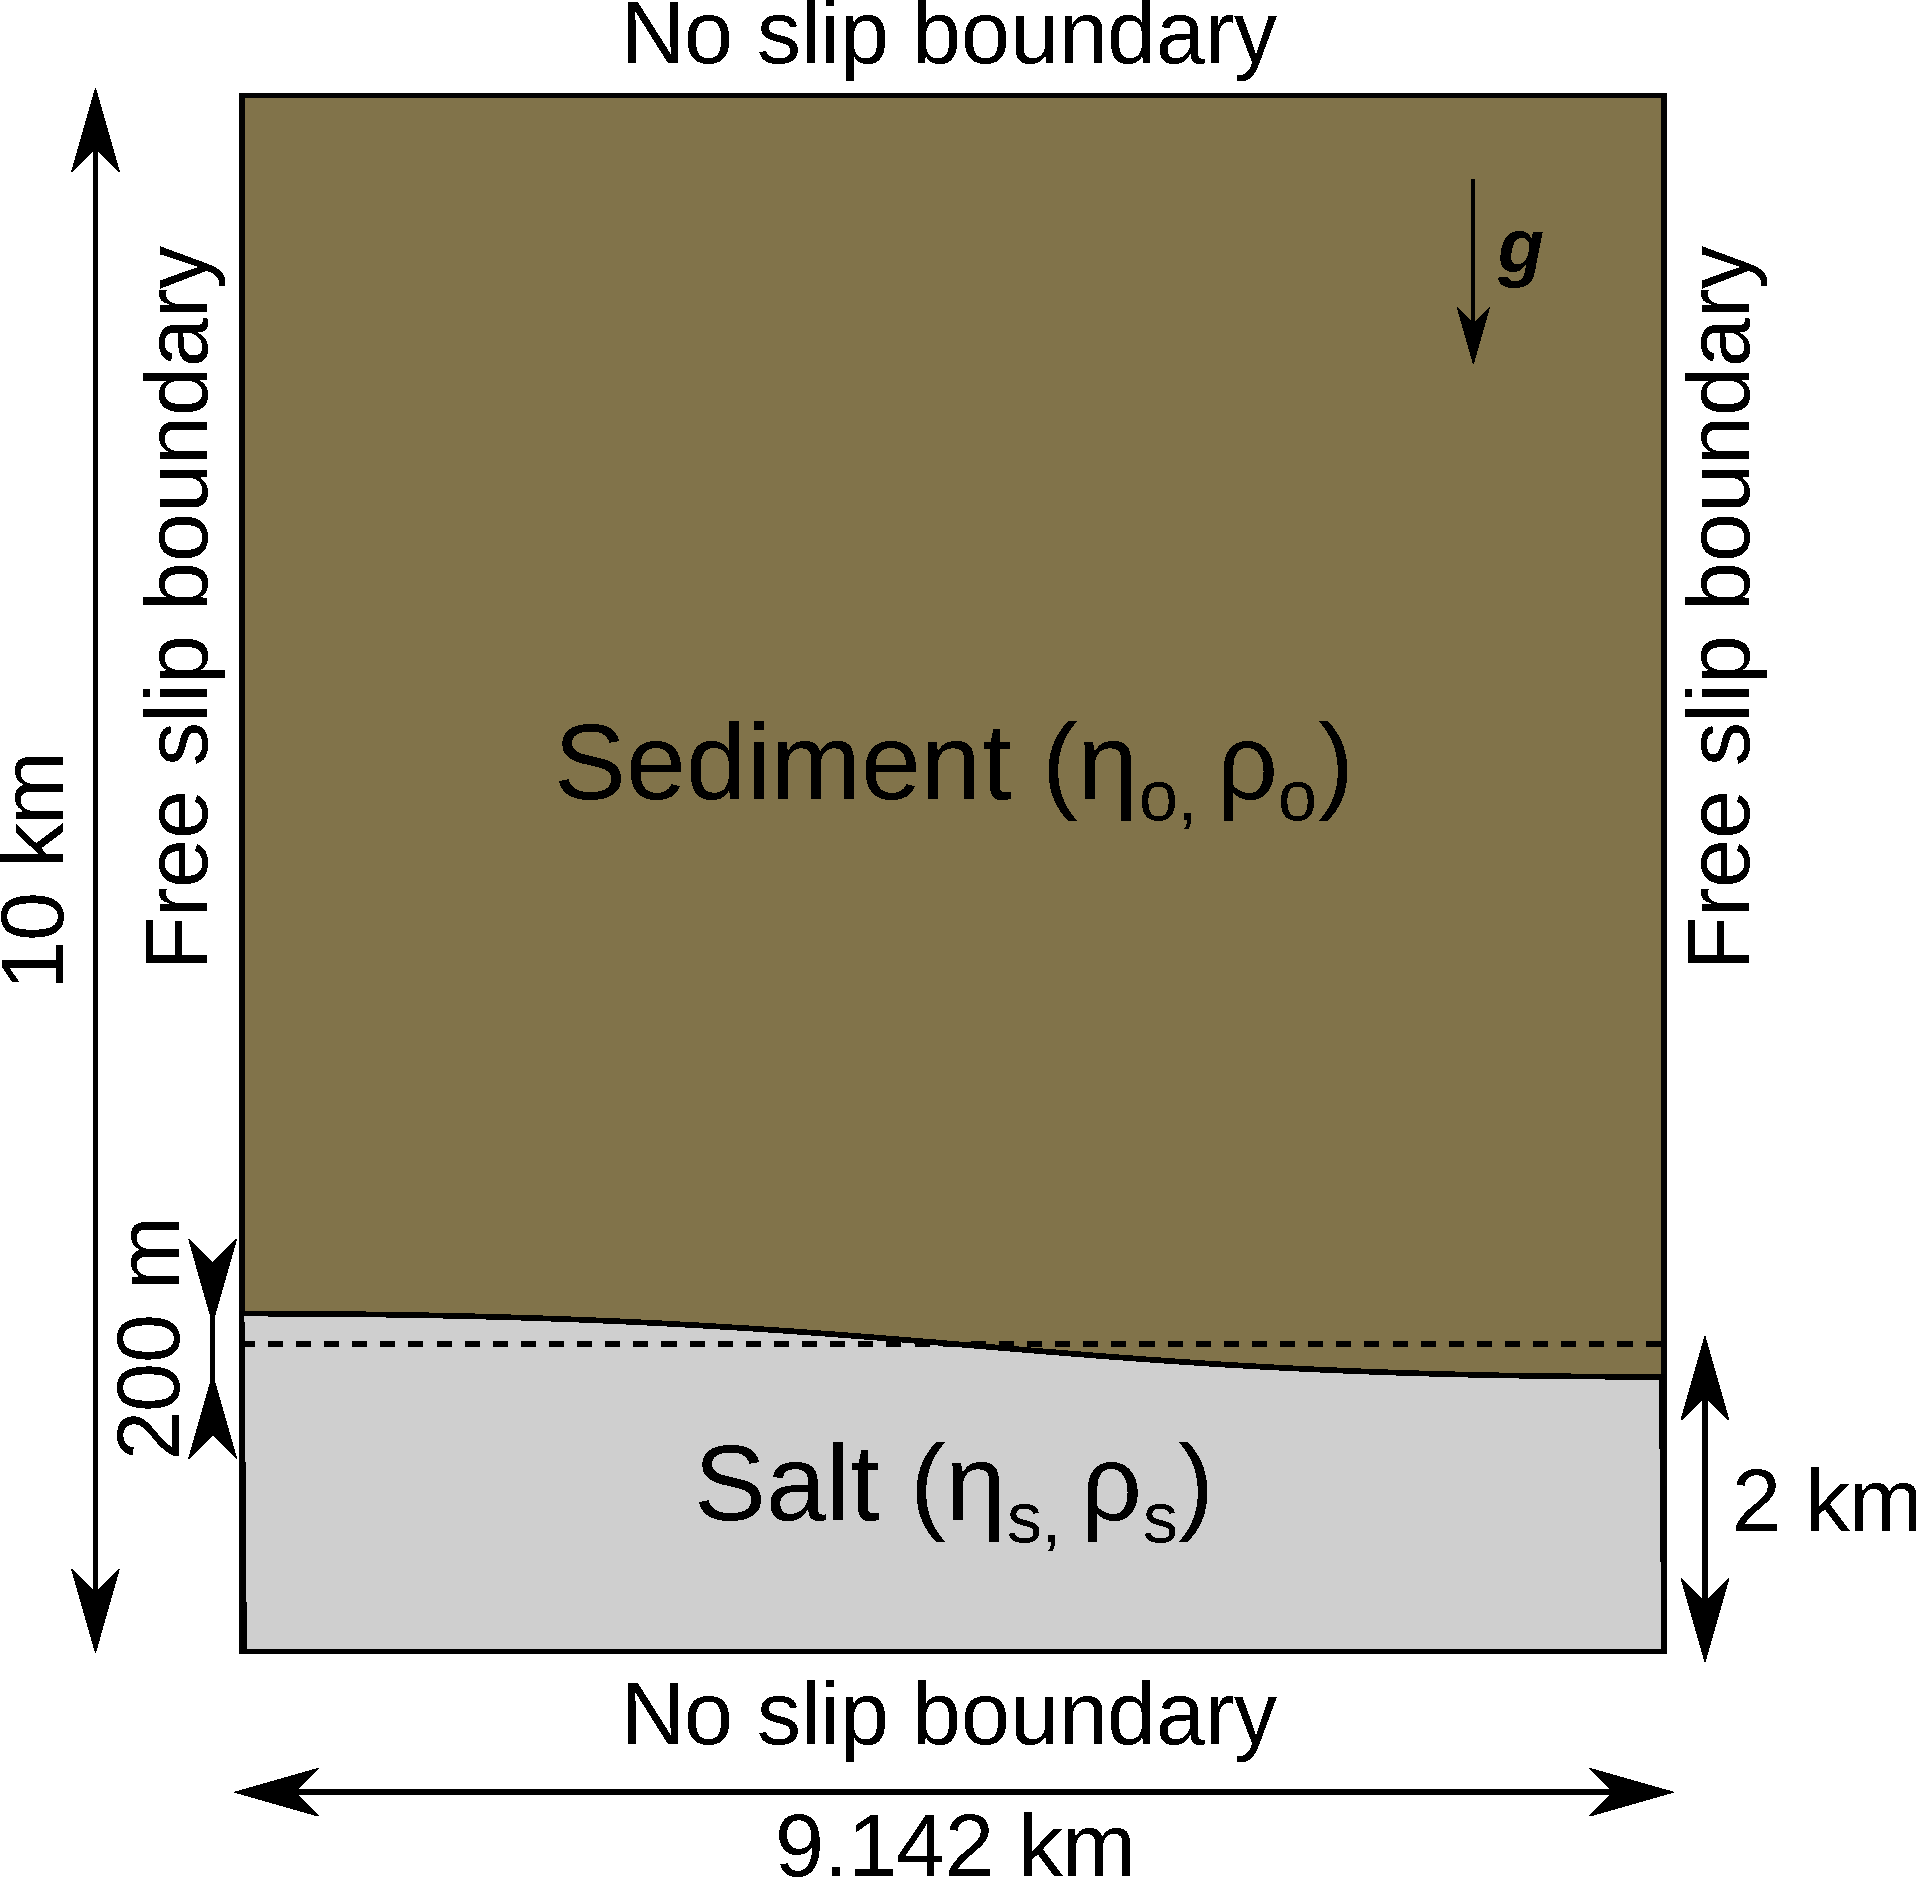
\includegraphics[width=7cm]{python_codes/fieldstone_41/images/setup}
\end{center}

Boundary conditions are no slip on the top and bottom, free slip on the sides.


In the original paper, 
length=1, viscosity=100, gravity =10, density contrast =10 and time unit =1,
so the dimensionless quantity
\[
\frac{\eta}{\delta\rho \cdot g \; length \cdot time} = \frac{100}{10 \cdot 10 \cdot 1 \cdot 1} =1
\]
If we now run a geometrically similar experiment with 
length=10km, viscosity=$10^{19}$, gravity=10, density contrast=450 and time unit = $t$
then we should also have 
\[
\frac{\eta}{\delta\rho \cdot g \; length \cdot time} = \frac{10^{19}}{450 \cdot 10 \cdot 10^4 \cdot t} =1
\]
i.e.,
\[
t = \frac{10^{14}}{450} \simeq 2.222 \cdot 10^{11}\text{s}
\]
This means that in order to plot our results against those in van Keken et al, their results
must be scaled: times must be multiplied by $t$ and velocities divided by 
$t/length = 2.222 \cdot 10^{7}\text{m/s}$  

The initial mass of the system is:
\[
M(t=0) = L_x \times 2km \times \rho_s + Lx \times 8km \times \rho_0 = 
9142 \cdot(2000\cdot 2150 + 8000\cdot 2600) \simeq 2.294642\cdot 10^{11}\text{kg}
\]

\paragraph{The code} It is based on stable $Q_2\times Q_1$ elements for the Stokes equations and 
the heat transport equation need not be solved. 
It relies on the Particle-in-Cell method (see Section~\ref{ss:pic}) for material advection. 
At startup {\tt nmarker\_per\_dim**2} particles are regularly placed in each element. 
There are in total:
\begin{lstlisting}
nmarker=nmarker_per_element*nel
\end{lstlisting}

Markers track material number, i.e. 1 or 2:
\begin{lstlisting}
for im in range (0,nmarker):
    if swarm_y[im]>salt_thickness+amplitude*np.cos(np.pi*swarm_x[im]/Lx):
       swarm_mat[im]=2
    else:
       swarm_mat[im]=1
\end{lstlisting}

Marker density is interpolated onto the Q1 mesh by means of the Q1 shape functions:
\begin{lstlisting}
for im in range(0,nmarker):
    ielx=int(swarm_x[im]/Lx*nelx)
    iely=int(swarm_y[im]/Ly*nely)
    iel=nelx*(iely)+ielx
    N1=0.25*(1-swarm_r[im])*(1-swarm_s[im])
    N2=0.25*(1+swarm_r[im])*(1-swarm_s[im])
    N3=0.25*(1+swarm_r[im])*(1+swarm_s[im])
    N4=0.25*(1-swarm_r[im])*(1+swarm_s[im])
    rho_nodal[iconP[0,iel]]+=rho_mat[swarm_mat[im]-1]*N1
    rho_nodal[iconP[1,iel]]+=rho_mat[swarm_mat[im]-1]*N2
    rho_nodal[iconP[2,iel]]+=rho_mat[swarm_mat[im]-1]*N3
    rho_nodal[iconP[3,iel]]+=rho_mat[swarm_mat[im]-1]*N4
    rho_nodal_counter[iconP[0,iel]]+=N1
    rho_nodal_counter[iconP[1,iel]]+=N2
    rho_nodal_counter[iconP[2,iel]]+=N3
    rho_nodal_counter[iconP[3,iel]]+=N4
rho_nodal/=rho_nodal_counter
\end{lstlisting}
This is a marker-centric approach, which is identical to the 
somewhat more instinctive node-centric approach which itself is similar
to the meshless methods approach (think of the SPH method kernel but with a 
square support). Density is later on interpolated onto the quadrature points 
with the $Q_1$ shape functions again to avoid the problems highlighted in 
Section~\ref{ss:bern}.
Viscosity is averaged per element by means of an arithmetic, geometric or harmonic mean.

Particles are advected by means of a (space) Runge-Kutta 1st/2nd/3rd order algorithm (see
Section~\ref{ss:rkm}). The time step $\delta t$ is set by means of the CFL criterion (see
Section~\ref{ss:cfl}).

The root mean square velocity and total mass of the system are computed every time step.

Simulations end when the maximum number of time steps is reached or when 
an element does not contain any particle.
\begin{center}
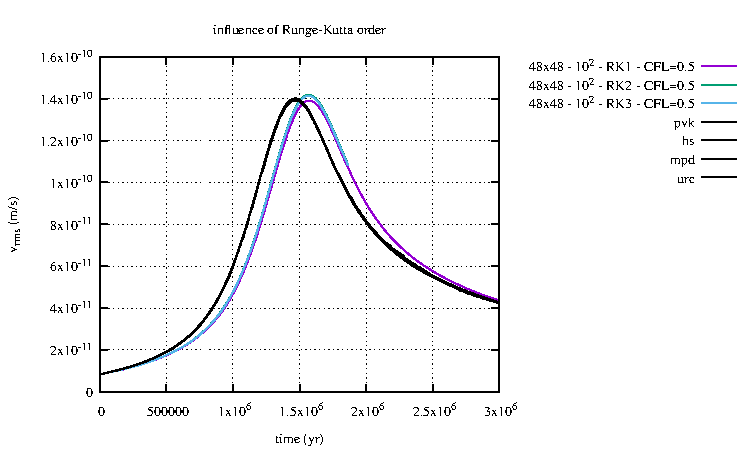
\includegraphics[width=7cm]{python_codes/fieldstone_41/results/vrms_RK.pdf}
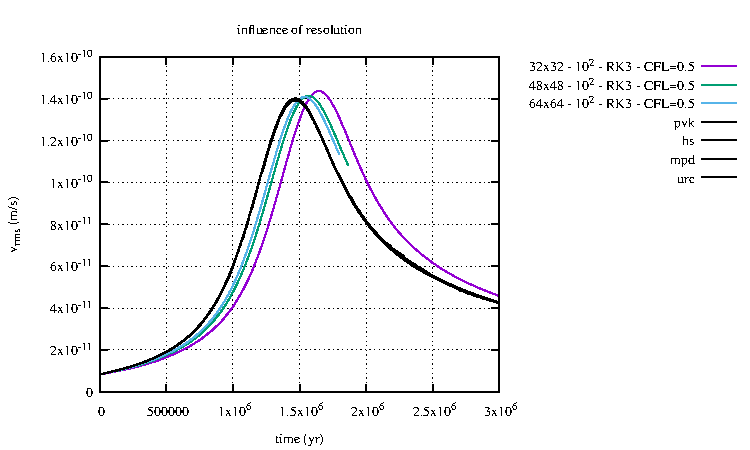
\includegraphics[width=7cm]{python_codes/fieldstone_41/results/vrms_RES.pdf}\\
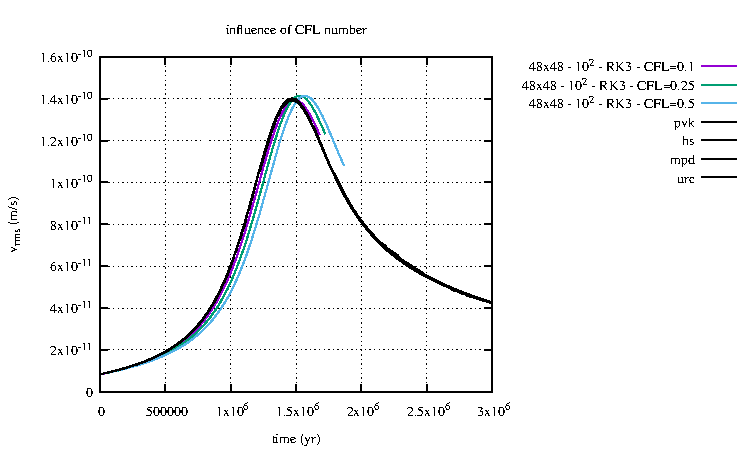
\includegraphics[width=7cm]{python_codes/fieldstone_41/results/vrms_CFL.pdf}
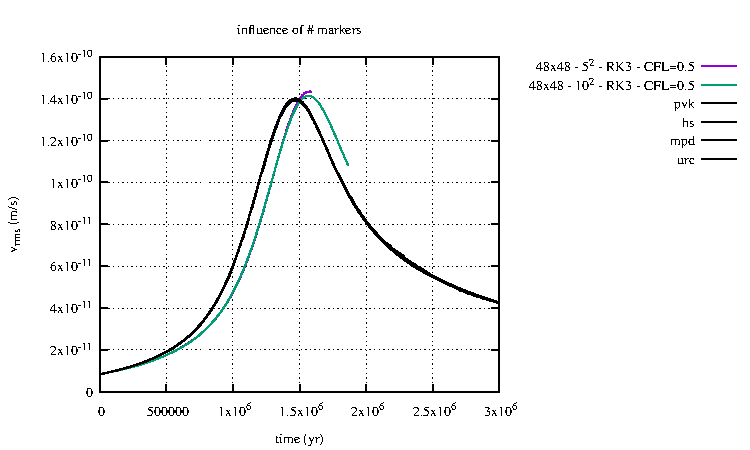
\includegraphics[width=7cm]{python_codes/fieldstone_41/results/vrms_nmarker.pdf}\\
{\captionfont Root mean square velocity as a function of time. Black curves are those in van Keken
et al (1997). Letters stand for authors initials.}
\end{center}



\begin{center}
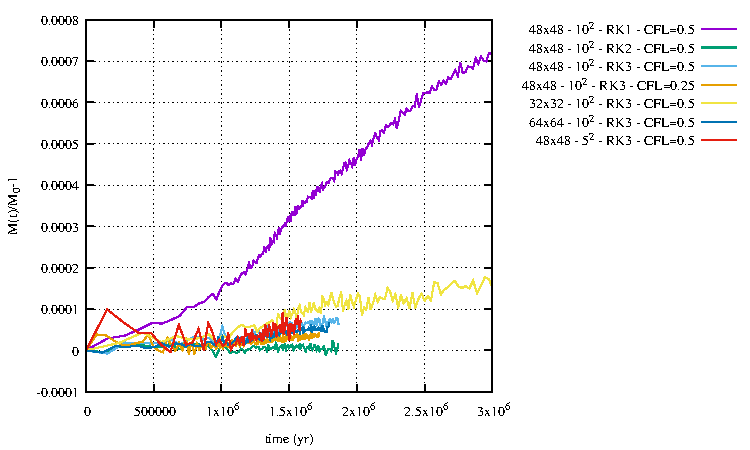
\includegraphics[width=7cm]{python_codes/fieldstone_41/results/mass.pdf}
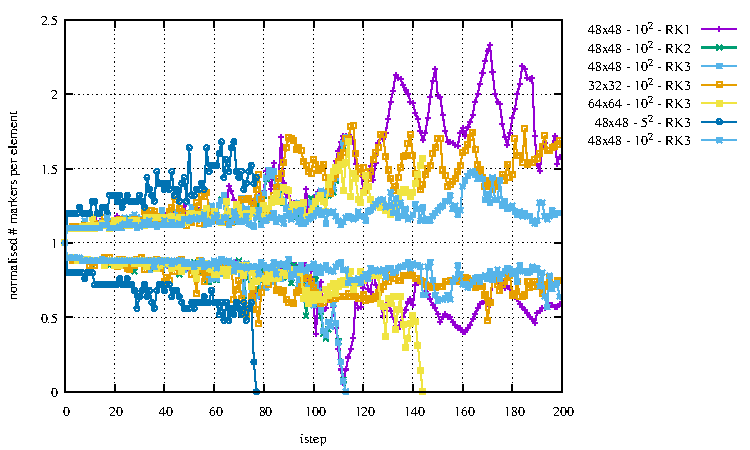
\includegraphics[width=7cm]{python_codes/fieldstone_41/results/nmarker.pdf}
\end{center}

\begin{center}
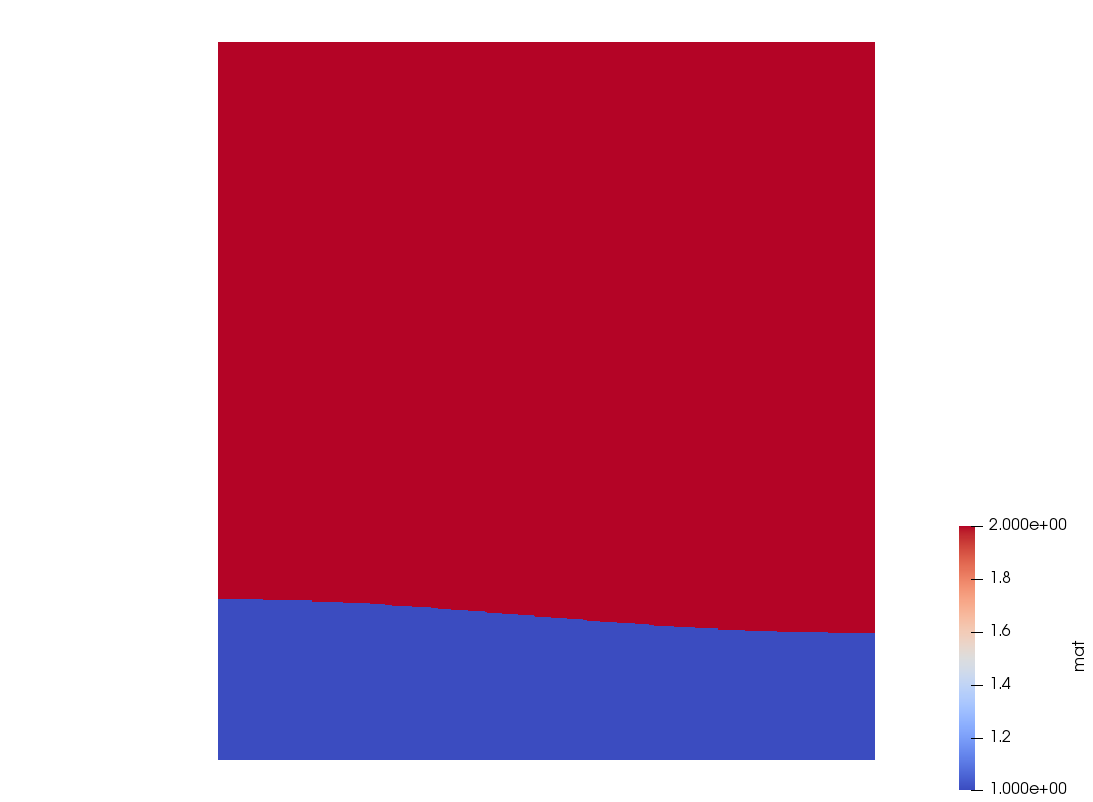
\includegraphics[width=5cm]{python_codes/fieldstone_41/results/64x64_10_RK3/markers0000}
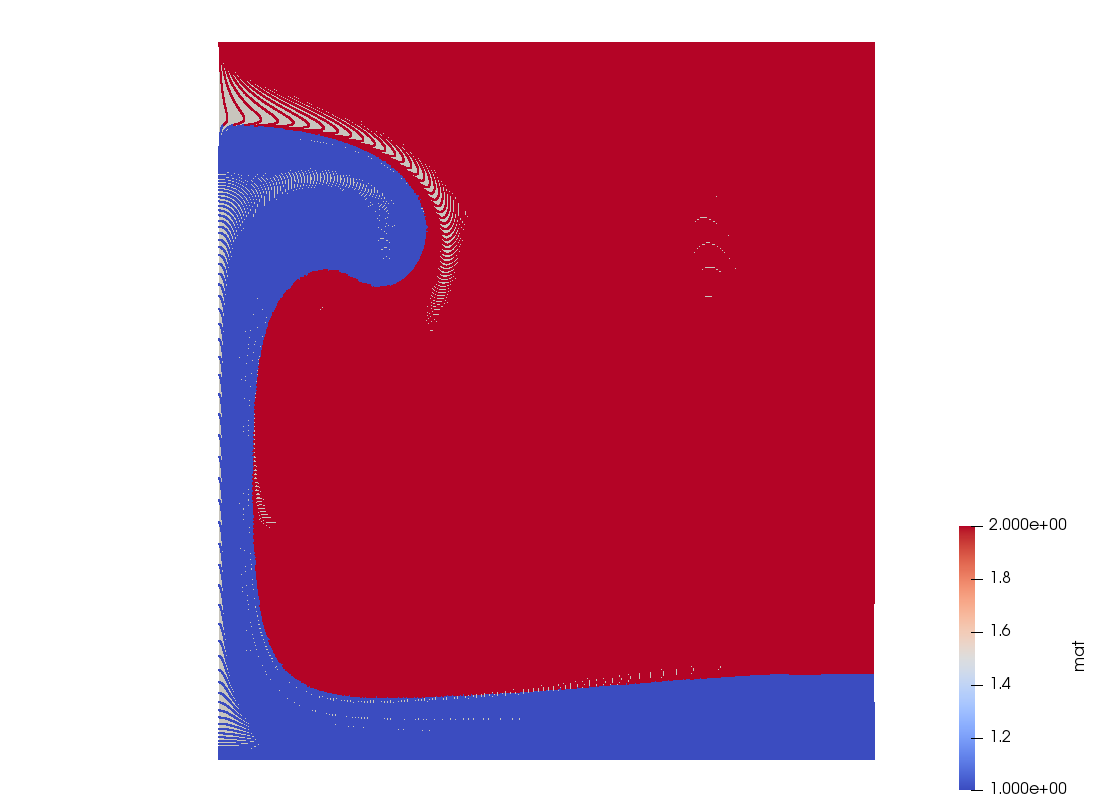
\includegraphics[width=5cm]{python_codes/fieldstone_41/results/64x64_10_RK3/markers0143}
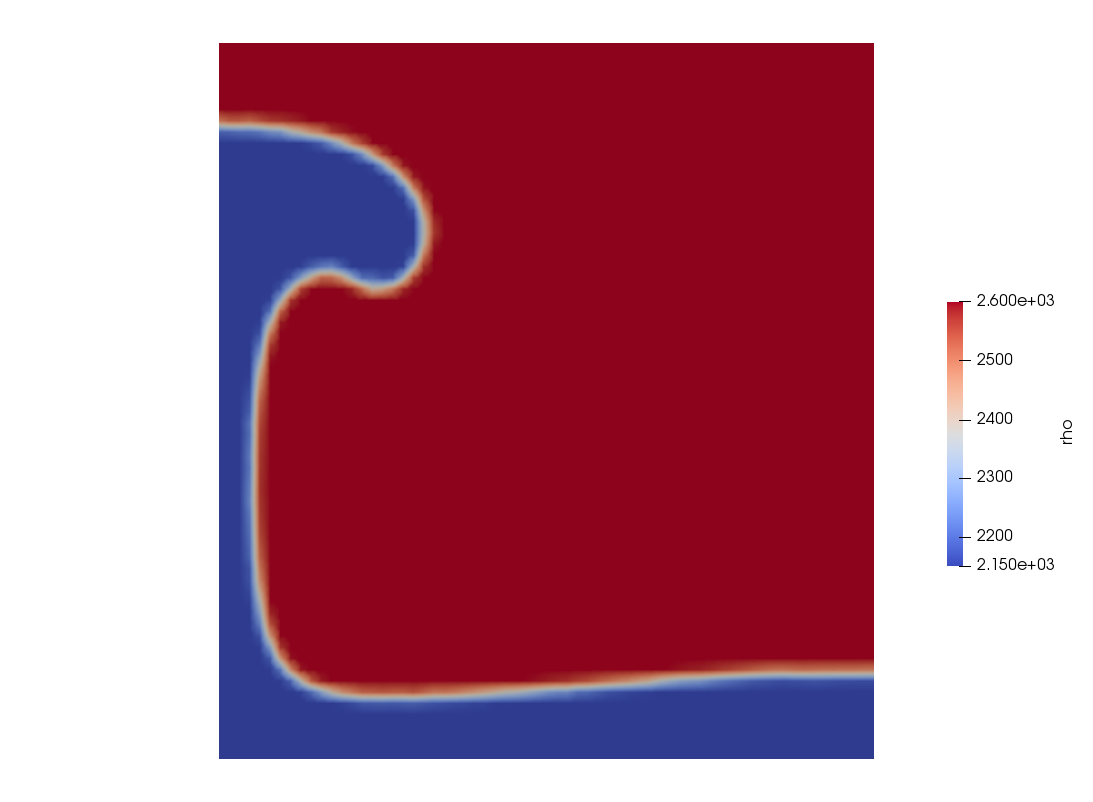
\includegraphics[width=5cm]{python_codes/fieldstone_41/results/64x64_10_RK3/rho_nodal_0143}\\
{\captionfont 64x64 simulation right before crash}
\end{center}




